% Intended LaTeX compiler: lualatex
\documentclass[xcolor=table,10pt,aspectratio=169]{beamer}

\RequirePackage[l2tabu,orthodox]{nag}            %% Warn about obsolete commands and packages
\RequirePackage{amsmath,amsfonts,amssymb,amsthm} %% Math
\RequirePackage{ifpdf,ifxetex,ifluatex}          %% Detect XeTeX and LuaTeX
\RequirePackage{xspace}
\RequirePackage{graphicx}
\RequirePackage{comment}
\RequirePackage{url}
\RequirePackage{relsize}
\RequirePackage{booktabs}
\RequirePackage{tabularx}
\RequirePackage[normalem]{ulem}
\ifluatex%
\else%
  \RequirePackage[all]{xy}
\fi%
\RequirePackage{etoolbox}
\RequirePackage{csquotes}
\RequirePackage[export]{adjustbox}

\RequirePackage{silence}
\WarningsOff[microtype]
\WarningFilter{microtype}{Unknown slot}

% https://tex.stackexchange.com/questions/64459/overfull-vbox-warning-disable
\vfuzz=30pt
\hfuzz=30pt


%%%
%%% Code Listings
%%%

\RequirePackage{listings}
\lstdefinelanguage{Sage}[]{Python}{morekeywords={True,False,sage,cdef,cpdef,ctypedef,self},sensitive=true}
\lstdefinelanguage{jupyter-python}[]{Python}{morekeywords={True,False,self},sensitive=true}

\lstset{frame=none,
  showtabs=False,
  showspaces=False,
  showstringspaces=False,
  commentstyle={\color{gray}},
  keywordstyle={\color{mLightBrown}\textbf},
  stringstyle ={\color{mDarkBrown}},
  frame=single,
  basicstyle=\tt\scriptsize\relax,
  backgroundcolor=\color{gray!190!black},
  inputencoding=utf8,
  literate={…}{{\ldots}}1,
  belowskip=0.0em,
}

\makeatletter
\patchcmd{\@verbatim}
  {\verbatim@font}
  {\verbatim@font\scriptsize}
  {}{}
\makeatother


%%%
%%% Pseudocode
%%%

\let\nl\undefine
\let\procedure\relax
\let\endprocedure\relax
\usepackage{algorithm2e}

%%%
%%% Tikz
%%%

\RequirePackage{tikz,pgfplots}
\pgfplotsset{compat=newest}

\usetikzlibrary{calc}
\usetikzlibrary{arrows}
\usetikzlibrary{automata}
\usetikzlibrary{positioning}
\usetikzlibrary{decorations.pathmorphing}
\usetikzlibrary{backgrounds}
\usetikzlibrary{fit,}
\usetikzlibrary{shapes.symbols}
\usetikzlibrary{chains}
\usetikzlibrary{shapes.geometric}
\usetikzlibrary{shapes.arrows}
\usetikzlibrary{graphs}

%% Cache but disable by default

\usetikzlibrary{external}
\tikzset{external/export=false}

\definecolor{DarkPurple}{HTML}{332288}
\definecolor{DarkBlue}{HTML}{6699CC}
\definecolor{LightBlue}{HTML}{88CCEE}
\definecolor{DarkGreen}{HTML}{117733}
\definecolor{DarkRed}{HTML}{661100}
\definecolor{LightRed}{HTML}{CC6677}
\definecolor{LightPink}{HTML}{AA4466}
\definecolor{DarkPink}{HTML}{882255}
\definecolor{LightPurple}{HTML}{AA4499}
\definecolor{DarkBrown}{HTML}{604c38}
\definecolor{DarkTeal}{HTML}{23373b}
\definecolor{LightBrown}{HTML}{EB811B}
\definecolor{LightGreen}{HTML}{14B03D}
\definecolor{DarkOrange}{HTML}{FFDD00}

\pgfplotsset{width=1.0\textwidth,
  height=0.6\textwidth,
  cycle list={%
    solid,LightGreen,thick\\%
    dotted,LightRed,very thick\\%
    dashed,DarkBlue,thick\\%
    dashdotted,DarkPink,thick\\%
    dashdotdotted,LightGreen,thick\\%
    loosely dotted,very thick\\%
    loosely dashed,DarkBlue,very thick\\%
    loosely dashdotted,DarkPink,very thick\\%
    \\%
    DarkBrown,thick\\%
  },
  legend pos=north west,
  legend cell align={left}}

\pgfplotsset{select coords between index/.style 2 args={
    x filter/.code={
        \ifnum\coordindex<#1\def\pgfmathresult{}\fi
        \ifnum\coordindex>#2\def\pgfmathresult{}\fi
    }
}}

\setlength{\marginparwidth}{2cm}
\pgfplotsset{compat=1.18}

%%%
%%% SVG (Inkscape)
%%%

\ifpdf% 
\providecommand{\executeiffilenewer}[3]{%
  \ifnum\pdfstrcmp{\pdffilemoddate{#1}}%
    {\pdffilemoddate{#2}}>0%
    {\immediate\write18{#3}}
  \fi%
}
\else%
\providecommand{\executeiffilenewer}[3]{%
  {\immediate\write18{#3}} % hack
}
\fi%

\providecommand{\includesvg}[2][1.0\textwidth]{%
 \executeiffilenewer{#1.svg}{#1.pdf}%
 {inkscape -z -D --file=#2.svg --export-pdf=#2.pdf --export-latex --export-area-page}%
 \def\svgwidth{#1} 
 \input{#2.pdf_tex}%
} 

%%%
%%% Attachments
%%%

\RequirePackage{embedfile}


%%%
%%% Metropolis Theme
%%%

\usetheme{metropolis}
\metroset{color/block=fill}
\metroset{numbering=none}
\metroset{outer/progressbar=foot}
\metroset{titleformat=smallcaps}

\setbeamercolor{description item}{fg=mLightBrown}
\setbeamerfont{footnote}{size=\scriptsize}
\setbeamercolor{example text}{fg=mDarkBrown}
\setbeamercolor{block title alerted}{fg=white, bg=mDarkBrown}
\setbeamerfont{alerted text}{series=\ifmmode\boldmath\else\bfseries\fi}

\definecolor{gamechangecolor}{HTML}{f8e8c6}

\renewcommand*{\UrlFont}{\ttfamily\relax}

%%%
%%% UTF-8 & Fonts
%%% 

% \RequirePackage{unicodesymbols} % after metropolis which loads fontspec

\ifboolexpr{bool{xetex} or bool{luatex}}{%
\setmonofont[BoldFont={Cousine Bold},
             ItalicFont={Cousine Italic},
             BoldItalicFont={Cousine Bold Italic},
             Scale=0.9]{Cousine}             
}{%
}

%%%
%%% BibLaTeX
%%%

\RequirePackage[backend=bibtex,
            style=alphabetic,
            maxnames=8,maxbibnames=8,maxalphanames=8,
            citestyle=alphabetic]{biblatex}

\bibliography{local.bib,abbrev3.bib,crypto_crossref.bib,rfc.bib,jacm.bib,dcc.bib}

\setbeamertemplate{bibliography item}[text]
% https://tex.stackexchange.com/questions/683533/beamer-theme-metropolis-does-not-allow-different-font-size-for-fullcite
\setbeamerfont{bibliography entry title}{size=}
\setbeamerfont{bibliography entry author}{size=}
\setbeamerfont{bibliography entry location}{size=}
\setbeamerfont{bibliography entry note}{size=}

\DeclareFieldFormat{title}{\alert{#1}}
\DeclareFieldFormat[book]{title}{\alert{#1}}
\DeclareFieldFormat[thesis]{title}{\alert{#1}}
\DeclareFieldFormat[inproceedings]{title}{\alert{#1}}
\DeclareFieldFormat[incollection]{title}{\alert{#1}}
\DeclareFieldFormat[article]{title}{\alert{#1}}
\DeclareFieldFormat[misc]{title}{\alert{#1}}

%%% 
%%% Microtype
%%%

\IfFileExists{upquote.sty}{\RequirePackage{upquote}}{}
%% https://github.com/schlcht/microtype/issues/43
%% \IfFileExists{microtype.sty}{\RequirePackage{microtype}}{}
%% \IfFileExists{microtype.sty}{\PassOptionsToPackage{verbose=silent}{microtype}}{}

\setlength{\parindent}{0pt}                   %%
\setlength{\parskip}{6pt plus 2pt minus 1pt}  %%
\setlength{\emergencystretch}{3em}            %% prevent overfull lines
\setcounter{secnumdepth}{0}                   %%

%%%
%%% Maths
%%%

\DeclareMathOperator{\Vol}{Vol}
\DeclareMathOperator{\vol}{vol}
\DeclareMathOperator{\GH}{GH}
\renewcommand{\vec}[1]{\ensuremath{\mathbf{#1}}\xspace}
\newcommand{\norm}[1]{\left\lVert#1\right\rVert}
\providecommand{\mat}[1]{\ensuremath{\vec{#1}}\xspace}
\providecommand{\ring}[0]{\ensuremath{\mathcal{R}}\xspace}


\usepackage{amsmath}
\usepackage{fontspec}
\usepackage{graphicx}
\usepackage{longtable}
\usepackage{wrapfig}
\usepackage{rotating}
\usepackage[normalem]{ulem}
\usepackage{capt-of}
\usepackage{hyperref}
\usepackage{booktabs}
\usepackage{newunicodechar}
\usepackage[notions,operators,sets,keys,ff,adversary,primitives,complexity,asymptotics,lambda,landau,advantage]{cryptocode}
\usepackage[capitalize]{cleveref}
\usepackage[,]{stmaryrd}
\usepackage[english]{babel}
\usepackage{xspace}
\usepackage{units}
\usepackage{nicefrac}
\usepackage{gensymb}
\usepackage{amsthm}
\usepackage{amsmath}
\usepackage{amssymb}
\usepackage{xcolor}
\usepackage{listings}
\usepackage[color=cyan!0!magenta!4!yellow!16]{todonotes}
\PassOptionsToPackage{british}{babel}
\setbeamerfont{alerted text}{series=\ifmmode\boldmath\else\bfseries\fi}
\definecolor{gamechangecolor}{HTML}{f8e8c6}
\definecolor{BrightOrange}{HTML}{f8e8c6}
\tikzexternalize[prefix=tikz-figures/]
\usetikzlibrary{trees}
\newcommand{\Ldis}{\ensuremath{\mathcal{L}_{\mathbf{s},\chi}}\xspace}
\newcommand{\rhf}{{\ensuremath{\sqrt{\alpha_{\beta}}}\xspace}}
\newcommand{\KeyGen}{\ensuremath{\mathsf{KeyGen}}\xspace}
\newcommand{\Enc}{\ensuremath{\mathsf{Enc}}\xspace}
\newcommand{\Dec}{\ensuremath{\mathsf{Dec}}\xspace}
\newcommand{\Encap}{\ensuremath{\mathsf{Encap}}\xspace}
\newcommand{\Decap}{\ensuremath{\mathsf{Decap}}\xspace}
\newcommand{\Sig}{\ensuremath{\Sigma}\xspace} %signature alg
\newcommand{\Sign}{\ensuremath{\mathsf{Sign}}\xspace}
\newcommand{\Verify}{\ensuremath{\mathsf{Verify}}\xspace}
\institute{\begin{columns} \begin{column}{0.55\columnwidth} ``\,`Cryptographers seldom sleep well' (Silvio Micali). Their careers are frequently based on very precise complexity-theoretic assumptions, which could be shattered the next morning. \textbf{A polynomial time algorithm for factoring would certainly prove more crushing than any paltry fluctuation of the Dow Jones.}'' -- \cite{STOC:Kilian88} \end{column} \begin{column}{0.35\columnwidth} \includegraphics[height=5\baselineskip]{Kings_Cryptographers_Logo.png} \end{column}\end{columns}}
\usetheme{default}
\author{Martin R. Albrecht}
\date{}
\title{Post-Quantum Cryptography, Lattices and \\ Learning with Errors}
\subtitle{A Primer}
\hypersetup{
pdfauthor={Martin R. Albrecht},
pdftitle={Post-Quantum Cryptography, Lattices and \\ Learning with Errors},
pdfkeywords={},
pdfsubject={},
pdfcreator={Emacs 30.2 (Org mode 9.7.34)},
pdflang={English},
colorlinks,
citecolor=gray,
filecolor=gray,
linkcolor=gray,
urlcolor=gray
}
\usepackage[backend=bibtex]{biblatex}

\begin{document}

\maketitle
\begin{frame}{Outline}
\tableofcontents
\end{frame}

\section{The Poverty of Public-Key Cryptography}
\label{sec:org09367c4}
\begin{frame}[label={sec:orgcc6988e}]{Cryptographic Primitives}
\textbf{Symmetric Primitives}

\begin{itemize}
\item Block and stream ciphers (AES, ChaCha20, \ldots)
\item Authentication codes (HMAC, Poly1305, \ldots)
\item Hash functions (SHA-2, SHA-3, \ldots)
\end{itemize}

\textbf{Asymmetric Primitives}

\begin{itemize}
\item Key agreement and public-key encryption (RSA, DH, ECDH, \ldots)
\item Digital signatures (RSA, DSA, ECDSA, \ldots)
\end{itemize}
\end{frame}
\begin{frame}[label={sec:org14e0157}]{The Poverty of Public-Key Cryptography}
\begin{center}
The Internet runs on factoring and discrete logarithms
\end{center}
\end{frame}
\begin{frame}[label={sec:org9074196}]{Rivest-Shamir-Adleman (RSA)}
\begin{columns}[t]
\begin{column}{0.5\columnwidth}
\begin{block}{Factoring}
Let \(p, q\) be primes of \(\secpar\) bits. Given \(n \coloneqq p \cdot q\), find \(p\).
\end{block}
\begin{block}{RSA}
Let \(n \coloneqq p\cdot q\) be the product of two \(\secpar\)-bit primes. Let \(e \nmid (p-1)\cdot(q-1)\). Given \(n, e\) and \(c \coloneqq m^{e} \bmod n\) for \(m \sample \ZZ_{n}\), find \(m\).
\end{block}
{\footnotesize \fullcite{RivShaAdl78} \par}
\end{column}
\begin{column}{0.5\columnwidth}
\begin{itemize}
\item We'd \alert{like} to say that RSA encryption/decryption is based on factoring, but such a reduction is not know
\begin{itemize}
\item If factoring is easy then RSA is insecure
\item RSA could be insecure and factoring hard\footnote{… on a classical computer, we'll get to that shortly}
\end{itemize}
\item Rabin encryption (\(\approx\) RSA with \(e=2\)) is based on factoring
\end{itemize}
\end{column}
\end{columns}
\end{frame}
\begin{frame}[label={sec:orgdfa8f6c}]{Diffie-Hellman (DH)}
\begin{columns}[t]
\begin{column}{0.5\columnwidth}
\begin{block}{Discrete Logarithms}
Let \(p\) be a \(\secpar\)-bit prime and let \(g\) be a generator of the multiplicative group \(\ZZ_{p}^{*}\). Given \(g^{a} \bmod p\) find \(a\).
\end{block}
\begin{block}{DH}
Let \(p\) be a \(\secpar\)-bit prime and let \(g\) be a generator of the multiplicative group \(\ZZ_{p}^{*}\). Given \(g^{a} \bmod p\), \(g^{b} \bmod p\) and \(u\), decide if \(u = g^{ab}\) or random.
\end{block}
{\footnotesize \fullcite{DifHel76} \par}
\end{column}
\begin{column}{0.5\columnwidth}
\begin{itemize}
\item We'd \alert{like} to say that the DH key exchange is based on discrete logarithms, but such a reduction is not known
\begin{itemize}
\item If discrete logs are easy, DH is insecure
\item DH could be easy and discrete logarithms hard\footnote{… on a classical computer, we'll get to that shortly}
\end{itemize}
\end{itemize}
\end{column}
\end{columns}
\end{frame}
\begin{frame}[label={sec:org9a9e72e}]{Diffie-Hellman (DH)}
\begin{itemize}
\item We didn't use any properties of \(\ZZ_{p}^{*}\) except that it is a group where discrete logarithms are hard.
\item Elliptic curves are also groups where it is believed to be hard to compute discrete logarithms\footnote{on a classical computer …}
\begin{itemize}
\item Indeed, it is believed only generic algorithms apply, in contrast to \(\ZZ_{p}^{*}\) \(\Rightarrow\) much smaller parameters
\end{itemize}
\item Elliptic curves are usually written additively and not multiplicative.
\end{itemize}
\end{frame}
\begin{frame}[label={sec:orgd159c0a}]{Diffie-Hellman (DH)}
\begin{columns}[t]
\begin{column}{0.5\columnwidth}
\begin{block}{Discrete Logarithms}
Let \(p\) be prime and let \(g\) be a generator of the multiplicative group \(\ZZ_{p}^{*}\). Given \(g^{a} \bmod p\) find \(a\).
\end{block}
\begin{block}{DH}
Let \(p\) be prime and let \(g\) be a generator of the multiplicative group \(\ZZ_{p}^{*}\). Given \(g^{a} \bmod p\), \(g^{b} \bmod p\) and \(u\), decide if \(u = g^{ab}\) or random.
\end{block}
\end{column}
\begin{column}{0.5\columnwidth}
\begin{block}{Discrete Logarithms}
Let \(\mathcal{G}\) be a group of order \(p\) and let \(G\) be a generator of \(\mathcal{G}\). Given \({a}\cdot G\) for \(a \in \ZZ_{p}\) find \(a\).\footnote{Here, \(a \cdot G\) means to add \(G\) to itself \(a\) times.}
\end{block}
\begin{block}{DH}
Let \(\mathcal{G}\) be a group of order \(p\) and let \(G\) be a generator of \(\mathcal{G}\). Given \((G, {a} \cdot G, {b} \cdot G, U)\) for \(a,b \in \ZZ_{p}\) decide if \(U = a\cdot b \cdot G\) or random in \(\mathcal{G}\).
\end{block}
\end{column}
\end{columns}
\end{frame}
\section{Post-Quantum Era}
\label{sec:org843ae8f}
\begin{frame}[label={sec:orga5b89b0}]{Quantum Computers}
\begin{itemize}
\item A quantum computer makes use of quantum effects (superpositions and entanglement) to perform computations.
\item Quantum computers are not \textbf{faster} than classical computers, they are \textbf{different}.
\item Some computations are easy on a quantum computer that are – as far as we know – hard on a classical computer.
\end{itemize}
\begin{columns}[t]
\begin{column}{0.5\columnwidth}
\begin{itemize}
\item Small universal quantum computers exist.
\item Key challenge is to scale them up by making them more stable.
\item There is a critical point where we can scale up further using error correction.
\end{itemize}
\end{column}
\begin{column}{0.4\columnwidth}
\begin{center}
\includegraphics[width=.9\linewidth]{./lecture-assumptions-google-72-qubit.png}
\end{center}
\end{column}
\end{columns}
\end{frame}
\begin{frame}[label={sec:org2132fc0}]{IBM Quantum Computing Timeline}
\begin{center}
\includegraphics[keepaspectratio,height=.8\textheight]{./lecture-assumptions-IBM_Quantum_Developmen_&_Innovation_Roadmap_Explainer_2024-Update-03.jpg}
\end{center}

{\tiny \url{https://www.ibm.com/quantum/roadmap} \par}
\end{frame}
\begin{frame}[label={sec:org4c361b4}]{Landscape of Quantum Computing in 2025}
\begin{center}
\includegraphics[keepaspectratio,height=.8\textheight]{./lecture-assumptions-quantum-landscape.png}
\end{center}

{\tiny \url{https://sam-jaques.appspot.com/quantum\_landscape\_2025} \par}
\end{frame}
\begin{frame}[label={sec:orgc687bec}]{Symmetric Primitives: Quantum Computing Perspective (Good News)}
Best known quantum algorithms for attacking symmetric cryptography are based on Grover’s algorithm. 

\begin{itemize}
\item Search key space of size \(2^n\) in \(2^{n/2}\) operations: AES-256 \(\rightarrow\) 128 “quantum bits of security”.
\item Taking all costs into account: \(> 2^{152}\) classical operations for AES-256.\footfullcite{EC:JNRV20}
\item Assuming a max depth of \(2^{96}\) for a quantum circuit: overall AES-256 cost is \(\approx 2^{190}\).
\item Does not parallelise: have to wait for \(2^{X}\) steps, cannot buy \(2^{32}\) quantum computers and wait \(2^X / 2^{32}\) steps.
\end{itemize}
\end{frame}
\begin{frame}[label={sec:org1caa80b}]{``based on very precise complexity-theoretic assumptions, which could be shattered the next morning''}
\begin{center}
\includegraphics[keepaspectratio,height=.8\textheight]{./lecture-assumptions-shor-paper.png}
\end{center}
\end{frame}
\begin{frame}[label={sec:orgb069ac3}]{``based on very precise complexity-theoretic assumptions, which could be shattered the next morning''}
\begin{center}
\includegraphics[keepaspectratio,height=.8\textheight]{./lecture-assumptions-shor.jpg}
\end{center}
\end{frame}
\begin{frame}[label={sec:org101bdff}]{Post-Quantum Standardisation of Primitives}
\begin{description}
\item[{NIST}] \textbf{Post Quantum \sout{Competition} Process}
\item[{ETSI}] Cyber Working Group for Quantum Safe Cryptography
\item[{ISO}] WG2 Standing Document 8 (SD8): Survey
\item[{IETF}] Standardisation of \textbf{stateful} hash-based signatures, nothing further
\item[{CSA}] Quantum-safe Security Working Group: position papers
\item[{NIST}] \textbf{Post Quantum Process: Digital Signatures}
\end{description}

\pause
\begin{alertblock}{Bottom Line}
Essentially, everyone was waiting for NIST.
\end{alertblock}
\vspace{0.7em}
\end{frame}
\begin{frame}[label={sec:org6770a75},fragile]{NIST PQC \sout{Competition} Process}
 \textbf{Timeline}

\begin{center}
\begin{tabular}{ll}
\toprule
Submission & November 2017\\
Round 2 Selection & January 2019\\
Round 3 Selection & July 2020\\
Winners and Round 4 Selection & July 2022\\
3/4 Final Standards & August 2024\\
Additional KEM Standard & March 2025\\
Final Standard for Falcon & ???\\
\bottomrule
\end{tabular}

\end{center}

\vspace{1em}
\begin{columns}[t]
\begin{column}{0.5\columnwidth}
\textbf{“Key Establishment”/Key Encapsulation}

\begin{itemize}
\item \texttt{(pk,sk) ← KeyGen()}
\item \texttt{(c,k) ← Encap(pk)}
\item \texttt{k ← Decap(c,sk)}
\end{itemize}
\end{column}
\begin{column}{0.5\columnwidth}
\textbf{Digital Signature}

\begin{itemize}
\item \texttt{(vk,sk)  ← KeyGen()}
\item \texttt{s  ← Sig(m,sk)}
\item \texttt{\{0,1\}  ← Verify(vk,s,m)}
\end{itemize}
\end{column}
\end{columns}
\end{frame}
\begin{frame}[label={sec:org670ee16}]{NIST PQC Outcome}
\textbf{NIST selected:}

\begin{description}
\item[{Kyber}] A lattice-based KEM (MLWE Problem)
\item[{Dilithium}] A lattice-based signature scheme (MSIS/MLWE Problems)
\item[{Falcon}] A lattice-based signature scheme (NTRU Problem)
\item[{SPHINCS+}] A hash-based signature scheme
\item[{HQC}] A code-based KEM (decoding random quasi-cyclic codes)
\end{description}
\end{frame}
\section{Learning with Errors}
\label{sec:org6d8c186}
\begin{frame}[label={sec:org3a36eda},fragile]{``Small Elements'' mod \(q\)}
 \begin{itemize}
\item We can represent \(\ZZ_{q}\) with integers \(\{0, 1, \ldots, q-1\}\)
\item We can also represent \(\ZZ_{q}\) with integers \(\{-\lfloor q/2 \rfloor, -\lfloor q/2 \rfloor +1, \ldots, \lfloor q/2 \rfloor\}\)
\item Example:
\begin{lstlisting}[language=Python,numbers=none]
q = 17
K = GF(q)
[[e.lift() for e in K], [e.lift_centered() for e in K]]
\end{lstlisting}

\begin{table}[htbp]
\centering
\begin{tabular}{rrrrrrrrrrrrrrrrr}
\toprule
0 & 1 & 2 & 3 & 4 & 5 & 6 & 7 & 8 & 9 & 10 & 11 & 12 & 13 & 14 & 15 & 16\\
0 & 1 & 2 & 3 & 4 & 5 & 6 & 7 & 8 & -8 & -7 & -6 & -5 & -4 & -3 & -2 & -1\\
\bottomrule
\end{tabular}
\label{}

\end{table}

\item The latter representation is called ``centred'' or ``balanced''.
\item We often implicitly assume the ``centred'' representation.
\item We informally say that \(e \in \ZZ_{q}\) is ``small'' if its balanced representation is small in absolute value.
\end{itemize}
\end{frame}
\begin{frame}[label={sec:org06ee4ce}]{1-dim LWE (even easier than RSA)}
\begin{columns}[t]
\begin{column}{0.4\columnwidth}
\alert{KeyGen}

\begin{itemize}
\item Pick a prime \(q \approx 2^{10,000}\)
\item Pick a random integer \(s \in \ZZ_q\)
\item Pick about \(t=20,000\) random \(a_i \in \ZZ_q\) and small \(e_i \approx 2^{9,850}\)
\item Publish pairs \(a_i, c_i = a_i \cdot s + e_i \bmod \ZZ_q\)
\end{itemize}

\alert{Encrypt}  \(m \in \{0,1\}\)

\begin{itemize}
\item Pick \(b_i \in \{0,1\}\)
\item \(d_0 = \sum_{i=0}^{t-1} b_i \cdot a_i\)
\item \(d_1 = \lfloor \frac{q}{2} \rfloor \cdot m + \sum_{i=0}^{t-1} b_i \cdot c_i\)
\item Return \(d_0, d_1\)
\end{itemize}
\end{column}
\begin{column}{0.6\columnwidth}
\alert{Decrypt}

\begin{itemize}
\item Compute \(d = d_1 - d_0 \cdot s\)
\end{itemize}
\begin{align*}
  &=  \left\lfloor \frac{q}{2} \right\rfloor \cdot m + \sum_{i=0}^{t-1} b_i \cdot c_i - \sum_{i=0}^{t-1} b_i \cdot a_i \cdot s\\
  &=  \left\lfloor \frac{q}{2} \right\rfloor \cdot m + \sum_{i=0}^{t-1} b_i \cdot (a_i \cdot s + e_i) - \sum_{i=0}^{t-1} b_i \cdot a_i \cdot s\\
  &=  \left\lfloor \frac{q}{2} \right\rfloor \cdot m + \sum_{i=0}^{t-1} b_i \cdot  e_i 
\end{align*}
\begin{itemize}
\item Return 1 if \(|d| > q/4\) and 0 otherwise.
\end{itemize}
\end{column}
\end{columns}
\end{frame}
\begin{frame}[label={sec:org0da5cea}]{The Learning with Errors Problem (LWE)}
Given \((\vec{A},\vec{c})\) with \(\vec{c} \in \ZZ_q^{m}\), \(\vec{A} \in \ZZ_q^{m \times n}\), \(\vec{s} \in \ZZ_q^{n}\) and \alert{small \(\vec{e} \in \ZZ^{m}\)} is

\begin{align*}
\left(\begin{array}{c}
\\
\\
\\ 
\vec{c} \\
\\
\\
\\
\end{array} \right) = \left(
\begin{array}{ccc}
\leftarrow & n & \rightarrow \\
\\
\\ 
& \vec{A} & \\
\\
\\
\\
\end{array} \right) \times \left( \begin{array}{c}
\\
\vec{s} \\
\\
\end{array} \right) \alert{+ \left(
\begin{array}{c}
\\
\\
\\ 
\vec{e} \\
\\
\\
\\
\end{array} 
\right)}
\end{align*}

or \(\vec{c} \sample \mathcal{U}\left(\ZZ_q^{m}\right)\).
\end{frame}
\begin{frame}[label={sec:org5d17a84}]{A Fair Warning: Gaussian Distributions}
\begin{itemize}
\item In this talk I am ignoring the specifics of the distribution \(\chi\). That is, the only slide with the phrase ``Discrete Gaussian distribution'' is this slide.

\item In practice, \alert{for encryption} the shape of the error does not seem to matter much.

\item Ignoring the distribution allows to brutally simply proof sketches: almost all technical difficulty in these proofs derives from arguing about two distributions being close.
\end{itemize}
\end{frame}
\begin{frame}[label={sec:org8172370}]{Normal Form LWE}
\begin{columns}[t]
\begin{column}{0.5\columnwidth}
Consider
\begin{itemize}
\item \(\mat{A}_{i} \in \ZZ_q^{n \times n}\), \(\vec{s} \in \ZZ_q^n\), \(\alert{\alert{\vec{e}}}_{i} \sample \chi^n\),
\item \(\vec{c}_0 = \mat{A}_0 \cdot \vec{s} + \alert{\vec{e}}_0\) and
\item \(\vec{c}_1 = \vec{A}_1 \cdot \vec{s} + \alert{\vec{e}}_1\)
\item We have with high probability
\end{itemize}
\begin{align*}
\vec{c}' &= \vec{c}_1 - \mat{A}_1 \cdot \mat{A}_0^{-1} \cdot \vec{c}_0\\
   &= \vec{A}_1\cdot \vec{s} + \alert{\vec{e}}_1 -  \mat{A}_1 \cdot \mat{A}_0^{-1} (\mat{A}_0 \cdot \vec{s} + \alert{\vec{e}}_0)\\
   &= \vec{A}_1\cdot \vec{s} + \alert{\vec{e}}_1 -  \mat{A}_1 \cdot \vec{s} -  \mat{A}_1 \cdot \mat{A}_0^{-1} \cdot \alert{\vec{e}}_0\\
   &= - \mat{A}_1 \cdot \mat{A}_0^{-1} \cdot \alert{\vec{e}}_0 + \alert{\vec{e}}_1\\
   &= \mat{A}' \cdot \alert{\vec{e}}_0 + \alert{\vec{e}}_1
\end{align*}
\end{column}
\begin{column}{0.5\columnwidth}
\begin{itemize}
\item We might as well assume that our secret is also sampled from \(\chi\).

\item \fullcite{C:ACPS09}
\end{itemize}
\end{column}
\end{columns}
\end{frame}
\begin{frame}[label={sec:orga845899}]{Dimension/Modulus Trade-Off}
Consider \(\vec{a}, \alert{\vec{s}} \in \mathbb{Z}_{q}^{d}\) where \(\vec{s}\) is small, then
\[q^{d-1} \cdot \langle{\vec{a},\alert{\vec{s}}}\rangle \approx \left(\sum_{i=0}^{d-1} q^{i} \cdot a_{i}\right) \cdot \left(\sum_{i=0}^{d-1} q^{d-i-1} \cdot \alert{s}_{i}\right) \bmod q^{d} = \tilde{a} \cdot \tilde{s} \bmod q^{d}.\]
If there is an algorithm solving the problem in \(\ZZ_{q^d}\), we can solve the problem in \(\mathbb{Z}_{q}^d\). 
\begin{example}[\(\ZZ_{q^{2}}\)]\label{sec:orgc522665}
\vspace{-1em}
\[q\cdot \left(a_{0}\cdot \alert{s}_{0} + a_{1} \cdot \alert{s}_{1}\right) + a_{0} \cdot \alert{s}_{1} + q^{2} \cdot a_{1} \cdot \alert{s}_{0} \bmod q = \left(a_{0} + q\cdot a_{1}\right) \cdot (q\cdot \alert{s}_{0} + \alert{s}_{1})\]
\end{example}
\fullcite{STOC:BLPRS13}
\end{frame}
\section{Algebraic Variants}
\label{sec:org54ab877}

\begin{frame}[label={sec:org7edfada}]{LWE}
\[
\begin{pmatrix}c_{0} \\ c_{1} \\ c_{2} \\ c_{3} \\ c_{4} \\ c_{5} \\ c_{6} \\ c_{7}\end{pmatrix} = 
\begin{pmatrix}
a_{0,0} & a_{0,1} & a_{0,2} & a_{0,3} & a_{0,4} & a_{0,5} & a_{0,6} & a_{0,7}\\
a_{1,0} & a_{1,1} & a_{1,2} & a_{1,3} & a_{1,4} & a_{1,5} & a_{1,6} & a_{1,7}\\
a_{2,0} & a_{2,1} & a_{2,2} & a_{2,3} & a_{2,4} & a_{2,5} & a_{2,6} & a_{2,7}\\
a_{3,0} & a_{3,1} & a_{3,2} & a_{3,3} & a_{3,4} & a_{3,5} & a_{3,6} & a_{3,7}\\
a_{4,0} & a_{4,1} & a_{4,2} & a_{4,3} & a_{4,4} & a_{4,5} & a_{4,6} & a_{4,7}\\
a_{5,0} & a_{5,1} & a_{5,2} & a_{5,3} & a_{5,4} & a_{5,5} & a_{5,6} & a_{5,7}\\
a_{6,0} & a_{6,1} & a_{6,2} & a_{6,3} & a_{6,4} & a_{6,5} & a_{6,6} & a_{6,7}\\
a_{7,0} & a_{7,1} & a_{7,2} & a_{7,3} & a_{7,4} & a_{7,5} & a_{7,6} & a_{7,7}\\
\end{pmatrix} \cdot
\begin{pmatrix}s_{0} \\ s_{1} \\ s_{2} \\ s_{3} \\ s_{4} \\ s_{5} \\ s_{6} \\ s_{7}\end{pmatrix} +
\begin{pmatrix}e_{0} \\ e_{1} \\ e_{2} \\ e_{3} \\ e_{4} \\ e_{5} \\ e_{6} \\ e_{7}\end{pmatrix}
\]
\begin{block}{Performance}
Storage: \(\mathcal{O}(n^{2})\); Computation \(\mathcal{O}(n^{2})\)
\end{block}
\end{frame}
\begin{frame}[label={sec:org07fecd5}]{Ring-LWE/Polynomial-LWE}
\[
\begin{pmatrix}c_{0} \\ c_{1} \\ c_{2} \\ c_{3} \\ c_{4} \\ c_{5} \\ c_{6} \\ c_{7}\end{pmatrix} = 
\begin{pmatrix}
\alert{a_{0}} & -a_{7} & -a_{6} & -a_{5} & -a_{4} & -a_{3} & -a_{2} & -a_{1} \\
\alert{a_{1}} & a_{0} & -a_{7} & -a_{6} & -a_{5} & -a_{4} & -a_{3} & -a_{2} \\
\alert{a_{2}} & a_{1} & a_{0} & -a_{7} & -a_{6} & -a_{5} & -a_{4} & -a_{3} \\
\alert{a_{3}} & a_{2} & a_{1} & a_{0} & -a_{7} & -a_{6} & -a_{5} & -a_{4} \\
\alert{a_{4}} & a_{3} & a_{2} & a_{1} & a_{0} & -a_{7} & -a_{6} & -a_{5} \\
\alert{a_{5}} & a_{4} & a_{3} & a_{2} & a_{1} & a_{0} & -a_{7} & -a_{6} \\
\alert{a_{6}} & a_{5} & a_{4} & a_{3} & a_{2} & a_{1} & a_{0} & -a_{7} \\
\alert{a_{7}} & a_{6} & a_{5} & a_{4} & a_{3} & a_{2} & a_{1} & a_{0}
\end{pmatrix}\cdot
\begin{pmatrix}s_{0} \\ s_{1} \\ s_{2} \\ s_{3} \\ s_{4} \\ s_{5} \\ s_{6} \\ s_{7}\end{pmatrix} +
\begin{pmatrix}e_{0} \\ e_{1} \\ e_{2} \\ e_{3} \\ e_{4} \\ e_{5} \\ e_{6} \\ e_{7}\end{pmatrix}
\]
\end{frame}
\begin{frame}[label={sec:org806ccb2}]{Ring-LWE/Polynomial-LWE}
\begin{align*}
\sum_{i=0}^{n-1} c_{i} \cdot X^{i} &= \left(\sum_{i=0}^{n-1} a_{i} \cdot X^{i}\right) \cdot \left(\sum_{i=0}^{n-1} s_{i} \cdot X^{i}\right) + \sum_{i=0}^{8} e_{i} \cdot X^{i} \bmod X^{n} +1\\
c(X) &= a(X) \cdot s(X) + e(X) \bmod \phi(X)
\end{align*}
\begin{block}{Performance (\(n\) is a power of two)}
Storage: \(\mathcal{O}(n)\); Computation \(\mathcal{O}(n \log n)\)
\end{block}
{\footnotesize \fullcite{AC:SSTX09} \par}

{\footnotesize \fullcite{EC:LyuPeiReg10} \par}
\end{frame}
\begin{frame}[label={sec:orgbc8779b}]{Module-LWE}
\[
\begin{pmatrix}c_{0,0} \\ c_{0,1} \\ c_{0,2} \\ c_{0,3} \\ c_{1,0} \\ c_{1,1} \\ c_{1,2} \\ c_{1,3}\end{pmatrix} = 
\left(\begin{array}{rrrr|rrrr}
\alert{a_{0,0}} & -a_{0,3} & -a_{0,2} & -a_{0,1} & \alert{a_{1,0}} & -a_{1,3} & -a_{1,2} & -a_{1,1} \\
\alert{a_{0,1}} &  a_{0,0} & -a_{0,3} & -a_{0,2} & \alert{a_{1,1}} &  a_{1,0} & -a_{1,3} & -a_{1,2} \\
\alert{a_{0,2}} &  a_{0,1} &  a_{0,0} & -a_{0,3} & \alert{a_{1,2}} &  a_{1,1} &  a_{1,0} & -a_{1,3} \\
\alert{a_{0,3}} &  a_{0,2} &  a_{0,1} &  a_{0,0} & \alert{a_{1,3}} &  a_{1,2} &  a_{1,1} &  a_{1,0} \\
\hline
\alert{a_{2,0}} & -a_{2,3} & -a_{2,2} & -a_{2,1} & \alert{a_{3,0}} & -a_{3,3} & -a_{3,2} & -a_{3,1} \\
\alert{a_{2,1}} &  a_{2,0} & -a_{2,3} & -a_{2,2} & \alert{a_{3,1}} &  a_{3,0} & -a_{3,3} & -a_{3,2} \\
\alert{a_{2,2}} &  a_{2,1} &  a_{2,0} & -a_{2,3} & \alert{a_{3,2}} &  a_{3,1} &  a_{3,0} & -a_{3,3} \\
\alert{a_{2,3}} &  a_{2,2} &  a_{2,1} &  a_{2,0} & \alert{a_{3,3}} &  a_{3,2} &  a_{3,1} &  a_{3,0} \\
\end{array}\right)\cdot
\begin{pmatrix}s_{0} \\ s_{1} \\ s_{2} \\ s_{3} \\ s_{4} \\ s_{5} \\ s_{6} \\ s_{7}\end{pmatrix} +
\begin{pmatrix}e_{0} \\ e_{1} \\ e_{2} \\ e_{3} \\ e_{4} \\ e_{5} \\ e_{6} \\ e_{7}\end{pmatrix}
\]
\end{frame}
\begin{frame}[label={sec:orge473c59}]{Module-LWE}
\[
\begin{pmatrix} c_{0}(X) \\ c_{1}(X) \end{pmatrix} =
\begin{pmatrix} a_{0}(X) & a_{1}(X) \\ a_{2}(X) & a_{3}(X) \end{pmatrix} \cdot
\begin{pmatrix} s_{0}(X) \\ s_{1}(X) \end{pmatrix} +
\begin{pmatrix} e_{0}(X) \\ e_{1}(X) \end{pmatrix}
\]
\begin{block}{Performance (\(n\) is a power of two)}
Storage: \(\mathcal{O}(k^{2} \cdot n)\); Computation \(\mathcal{O}(k^{2} \cdot n \log n)\)
\end{block}
{\footnotesize \fullcite{Langlois:2015:WCA} \par}
\end{frame}
\section{LWE and Lattices}
\label{sec:orgcf8dfa0}
\begin{frame}[label={sec:org073d5b0},fragile]{Lattices}
\begin{columns}
\begin{column}{0.5\columnwidth}
\begin{itemize}
\item A lattice is a discrete subgroup of \(\RR^d\)
\item It can be written as
\[
  \Lambda = \left\{\sum_{i=0}^{d-1} v_i \cdot \vec{b}_i \mid v_i \in \ZZ\right\}
  \]
for some basis vectors \(\vec{b}_i\).
\item We write \(\Lambda(\mat{B})\) for the lattices spanned by the columns of \(\mat{B}\).
\item A lattice is \(q\)-ary if it contains \(q\,\ZZ^{d}\), e.g. \(\{\vec{x} \in \ZZ_{q}^{d} \mid \vec{x} \cdot \vec{A} \equiv \vec{0}\}\) for some \(\vec{A} \in \ZZ^{d \times d'}\).
\end{itemize}
\end{column}
\begin{column}{0.5\columnwidth}
\tikzset{external/export=true}
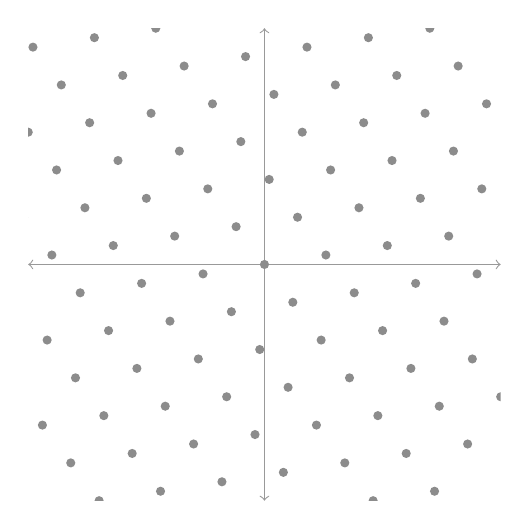
\begin{tikzpicture}

  \begin{scope}[scale=.6]
    \coordinate (Origin)   at (0,0);
    \coordinate (XAxisMin) at (-5,0);
    \coordinate (XAxisMax) at (5,0);
    \coordinate (YAxisMin) at (0,-5);
    \coordinate (YAxisMax) at (0,5);
    \draw [thin, black!40, <->] (XAxisMin) -- (XAxisMax);% Draw x axis
    \draw [thin, black!40,<->] (YAxisMin) -- (YAxisMax);% Draw y axis
    %\draw[style=help lines,dashed,black!20] (-5,-5) grid[step=1cm] (5,5);

    \begin{scope}
      \clip (-5,-5) rectangle (5,5); % Clips the picture...
      \pgftransformcm{1}{0.6}{0.7}{1}{\pgfpoint{0cm}{0cm}}

      % setup the nodes
      \foreach \x in {-15,...,15}
      \foreach \y in {-15,...,15}
      {
        \node[shape=circle,fill=black!45,scale=0.35] (\x-\y) at (2*\x,\y+3){};
      }
    \end{scope}
  \end{scope}

\end{tikzpicture}
\tikzset{external/export=false}

{\tiny Picture credit: David Wong }\par
\end{column}
\end{columns}
\end{frame}
\begin{frame}[label={sec:org20c30e1},fragile]{Shortest Vector Problem}
\begin{columns}
\begin{column}{0.5\columnwidth}
\begin{definition}
Given a lattice basis \(\mat{B}\), find a shortest non-zero vector in \(\Lambda(\mat{B})\).
\end{definition}

\begin{itemize}
\item The most natural problem on lattices
\item We write \(\lambda_{1}(\Lambda)\) for the Euclidean norm of a shortest vector.
\item NP-hard to solve exactly
\item Cryptography relies on approximate variants without such a reduction
\end{itemize}
\end{column}
\begin{column}{0.5\columnwidth}
\tikzset{external/export=true}
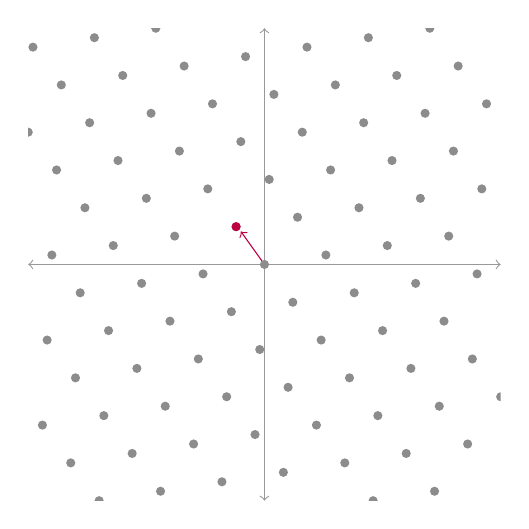
\begin{tikzpicture}
  \begin{scope}[scale=.6]
    \coordinate (Origin)   at (0,0);
    \coordinate (XAxisMin) at (-5,0);
    \coordinate (XAxisMax) at (5,0);
    \coordinate (YAxisMin) at (0,-5);
    \coordinate (YAxisMax) at (0,5);
    \draw [thin, black!40, <->] (XAxisMin) -- (XAxisMax);% Draw x axis
    \draw [thin, black!40,<->] (YAxisMin) -- (YAxisMax);% Draw y axis
    \draw [thin, purple,->] (0,0) -- (-.5,.7);
    % \draw[style=help lines,dashed,black!20] (-5,-5) grid[step=1cm] (5,5);

    \begin{scope}
      \clip (-5,-5) rectangle (5,5); % Clips the picture...
      \pgftransformcm{1}{0.6}{0.7}{1}{\pgfpoint{0cm}{0cm}}

      % setup the nodes
      \foreach \x in {-15,...,15}
      \foreach \y in {-15,...,15}
      {
        \node[shape=circle,fill=black!45,scale=0.35] (\x-\y) at (2*\x,\y+3){};
      }
    \end{scope}
    % our little node
    \node[shape=circle,fill=purple,scale=0.35] at (-.6,.8){};
  \end{scope}

\end{tikzpicture}
\tikzset{external/export=false}

{\tiny Picture credit: David Wong }\par
\end{column}
\end{columns}
\end{frame}
\begin{frame}[label={sec:org43edb22}]{Bounded Distance Decoding}
\begin{columns}
\begin{column}{0.5\columnwidth}
\begin{definition}
Given a lattice basis \(\mat{B}\), a vector \(\vec{t}\), and a parameter \(0 < \alpha\) such that the Euclidean distance \textnormal{dist}\((\vec{t},\vec{B}) < \alpha \cdot \lambda_{1}(\Lambda(\vec{B}))\), find the lattice vector \(\vec{v} \in \Lambda(\vec{B})\) which is closest to \(\vec{t}\).
\end{definition}

\begin{itemize}
\item When \(\alpha < 1/2\) unique decoding is guaranteed but for \(\alpha < 1\) we typically still expect unique decoding.
\item BDD is a special case of the Closest Vector Problem where there is no bound on the distance to the lattice.
\end{itemize}
\end{column}
\begin{column}{0.5\columnwidth}
\tikzset{external/export=true}
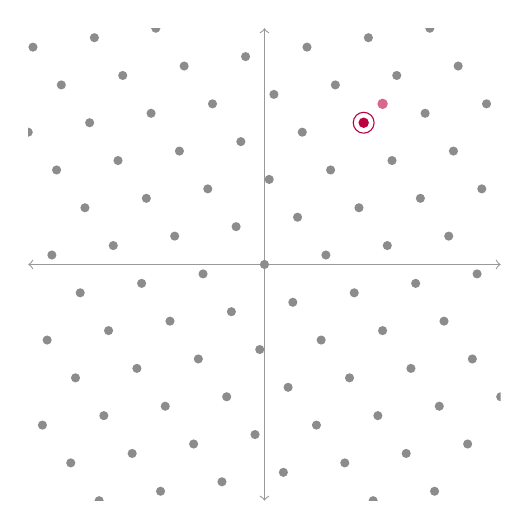
\begin{tikzpicture}

  \begin{scope}[scale=.6,shift={(12,0)}]
    \coordinate (Origin)   at (0,0);
    \coordinate (XAxisMin) at (-5,0);
    \coordinate (XAxisMax) at (5,0);
    \coordinate (YAxisMin) at (0,-5);
    \coordinate (YAxisMax) at (0,5);
    \draw [thin, black!40, <->] (XAxisMin) -- (XAxisMax);% Draw x axis
    \draw [thin, black!40,<->] (YAxisMin) -- (YAxisMax);% Draw y axis
    % \draw[style=help lines,dashed,black!20] (-5,-5) grid[step=1cm] (5,5);


    \begin{scope}
      \clip (-5,-5) rectangle (5,5); % Clips the picture...
      \pgftransformcm{1}{0.6}{0.7}{1}{\pgfpoint{0cm}{0cm}}

      % setup the nodes
      \foreach \x in {-15,...,15}
      \foreach \y in {-15,...,15}
      {
        \node[shape=circle,fill=black!45,scale=0.35] (\x-\y) at (2*\x,\y+3){};
      }
    \end{scope}

    % our little node
    \node[shape=circle,fill=purple!60,scale=0.4] at (2.5,3.4){};
    \node[shape=circle,fill=purple,scale=0.4] at (2.1,3){};
    \node[shape=circle,fill=none,draw=purple,scale=0.8] at (2.1,3){};

  \end{scope}

\end{tikzpicture}
\tikzset{external/export=false}

{\tiny Picture credit: David Wong }\par
\end{column}
\end{columns}
\end{frame}
\begin{frame}[label={sec:org18ac27b}]{LWE \textbf{is} Bounded Distance Decoding (BDD) on Random \(q\)-ary Lattices}
Let
\[
\mat{L} =  \begin{pmatrix}
    q\mat{I} & \mat{A}\\
    0 & \mat{I}\\
  \end{pmatrix}
\]
We can reformulate the matrix form of the LWE equation \(\vec{A} \cdot \vec{s} + \vec{e} \equiv \vec{c} \bmod q\) as a linear system over the Integers as:
\[
  \mat{L} \cdot
  \begin{pmatrix}
    \vec{*}\\
    \vec{s}
  \end{pmatrix} +
  \begin{pmatrix}
    \vec{e}\\
    -\vec{s}
  \end{pmatrix}  
 = 
  \begin{pmatrix}
    q\mat{I} & -\mat{A}\\
    0 & \mat{I}\\
  \end{pmatrix} \cdot
  \begin{pmatrix}
    \vec{*}\\
    \vec{s}
  \end{pmatrix} +
  \begin{pmatrix}
    \vec{e}\\
    -\vec{s}
  \end{pmatrix}  
= 
  \begin{pmatrix}
    \vec{c}\\
    \vec{0}
  \end{pmatrix}
\]

The vector \((\vec{c}^T, \vec{0}^T)^T\) is close to the lattice \(\Lambda\left(\mat{L}\right)\) with offset \((\vec{e}^T, -\vec{s}^T)^T\).
\end{frame}
\begin{frame}[label={sec:org41f81c1}]{Is that a Good Choice?}
\begin{itemize}
\item Maybe BDD on random \(q\)-ary lattices is easier than BDD in general?
\item Maybe BDD is easier than SVP?
\end{itemize}
\end{frame}
\begin{frame}[label={sec:org0701673}]{Sketch: BDD on Random \(q\)-ary Lattices solves BDD on any Lattice}
\begin{itemize}
\item We are given some basis \(\mat{B} \in \ZZ^{d \times d}\) and some target \(\vec{t}\) s.t. \(\vec{t} = \mat{B}\cdot \vec{s} + \vec{e}\) with \(\vec{e}\) small
\item Pick some large \(q \geq 2^{2d}\)
\item Sample some \(\mat{U}\) (see below)
\item Set \(\mat{A} = \mat{U}\cdot \mat{B} \bmod q\) and consider \(\vec{c} = \mat{U} \cdot \vec{t} + \vec{e}'\) with \({\vec{e}'}\) small
\begin{align*}
\vec{c} &= \mat{U} \cdot \vec{t} + \vec{e}' = \mat{U} \cdot \left(\mat{B}\cdot \vec{s} + \vec{e} \right) + \vec{e}' = \mat{U} \cdot \mat{B}\cdot \vec{s} + \mat{U} \cdot \vec{e} + \vec{e}' = \mat{A} \cdot \vec{s} + \vec{e}''
\end{align*}
\item We can pick \(\mat{U}\)
\begin{itemize}
\item large enough to make \(\mat{A}\) uniform mod \(q\) and
\item small enough to make \(\mat{U} \cdot \vec{e} + \vec{e}'\) small and well distributed
\end{itemize}
using ``smoothing parameter'' arguments on \(\Lambda(\mat{B}^{-T})\)
\end{itemize}

\fullcite{Regev:2009:LLE}
\end{frame}
\begin{frame}[label={sec:orga59761d}]{Sketch: Solving BDD on any Lattice implies solving GapSVP}
Say we want to decide if \(\lambda_{1}(\Lambda) \leq 1\) or \(\lambda_{1}(\Lambda) > \gamma\) and we have a BDD solver with \(\alpha = c\cdot \gamma\).

\begin{itemize}
\item Pick a random \(\vec{z} \in \Lambda\), add a small error \(\vec{e}\) of norm \(c\cdot \gamma\)
\item Run the BDD solver.
\item If it returns \(\vec{z}\) then output \(\lambda_{1}(\Lambda) > \gamma\), else output \(\lambda_{1}(\Lambda) \leq 1\).\footfullcite{STOC:Peikert09}
\end{itemize}

Regev showed: If you have a BDD solver you can find a short basis on a quantum computer. \footfullcite{Regev:2009:LLE}
\end{frame}
\begin{frame}[label={sec:org592ad5e},fragile]{Concrete Hardness: Cryptanalysis}
 \begin{itemize}
\item This tells us random \(q\)-ary lattices are not a terrible choice
\item To establish how long it actually takes to solve LWE, we rely on cryptanalysis

\begin{lstlisting}[language=Python,numbers=none]
from estimator import *
schemes.Kyber512
\end{lstlisting}

\phantomsection
\label{}
\begin{verbatim}
LWEParameters(n=512, q=3329, Xs=D(σ=1.22), Xe=D(σ=1.22), m=512, tag='Kyber 512')
\end{verbatim}


\begin{lstlisting}[language=Python,numbers=none]
LWE.primal_usvp(schemes.Kyber512)
\end{lstlisting}

\phantomsection
\label{}
\begin{verbatim}
rop: ≈2^143.8, red: ≈2^143.8, δ: 1.003941, β: 406, d: 998, tag: usvp
\end{verbatim}
\end{itemize}

\begin{center}
\url{https://github.com/malb/lattice-estimator/}
\end{center}
\end{frame}
\section{LWE Encryption}
\label{sec:orgf9ed2d8}
\begin{frame}[label={sec:org25fa90a}]{Convention}
\begin{itemize}
\item I am going to use the Ring-LWE formulation \[c_{i}(X) = a_{i}(X)\cdot s(X) + e_{i}(X)\]
Thus, each sample corresponds to ``\(n\) LWE samples''
\item I will suppress the ``\((X)\)'' in ``\(a(X)\)'' etc.
\item I will assume \(s\) is ``small'' and that the product of two ``small'' things is ``small''.
\item I will write \(\alert{e_{i}}\) to emphasise that \(e_{i}\) is small.
\end{itemize}
\begin{block}{TL;DR: I will write}
\[c_{i} = a_{i}\cdot \alert{s} + \alert{e_{i}}\]
\end{block}
\end{frame}
\begin{frame}[label={sec:org245ab3f}]{DH to Ring-LWE Dictionary}
\begin{center}
\begin{tabular}{ll}
\toprule
DH Land & Ring-LWE Land\\
\midrule
\(g\) & \(a\)\\
\(g^x\) & \(a\cdot {s} + \alert{e}\)\\
 & \\
\(g^x \cdot g^y = g^{x+y}\) & \((a\cdot {s} + \alert{e_0}) + (a \cdot {t} + \alert{e_1}) = a \cdot {(s+t)} + \alert{e'}\)\\
 & \\
\((g^a)^b = (g^b)^a\) & \((a\cdot \alert{s} + \alert{e})\cdot \alert{t} = (a\cdot \alert{s} \cdot \alert{t} + \alert{e} \cdot \alert{t})\)\\
 & \(\approx a\cdot \alert{s} \cdot \alert{t} \approx (a\cdot \alert{t} + \alert{e})\cdot \alert{s}\)\\
 & \\
\((g, g^a, g^b, g^{ab})\) & \((a,\ a\cdot \alert{s} + \alert{e},\ a\cdot \alert{t} + \alert{d},\ a \cdot \alert{s} \cdot \alert{t} + \alert{e'})\)\\
\(\approx_c (g, g^a, g^b, u)\) & \(\approx_c (a,\ a\cdot \alert{s} + \alert{e},\ a\cdot \alert{t} + \alert{d},\ u)\)\\
\bottomrule
\end{tabular}

\end{center}
\end{frame}
\begin{frame}[label={sec:org66ae477}]{Regev's Encryption Scheme}
You have already seen it.

\begin{description}
\item[{KeyGen}] Publish \(c_{i} = a_{i} \cdot s + \alert{e_{i}}\) for \(i=0,\ldots, \lceil 2\, n \log q\rceil\)
\item[{Encrypt}] \[d_{0} = \sum \alert{b_{i}} \cdot a_{i},\quad  d_{1} = \left(\sum \alert{b_{i}} \cdot c_{i} \right) + \lfloor q/2 \rfloor \cdot m  \textnormal{ with } \alert{b_{i}} \in \bin, m \in \bin^{n}\]
\item[{Decrypt}] \begin{align*}
\left\lfloor \frac{2}{q} \cdot \left(d_{1} - d_{0} \cdot s\right) \right\rceil &= \left\lfloor \frac{2}{q} \cdot \left(\left(\sum \alert{b_{i}} \cdot c_{i} \right) + \left\lfloor \frac{q}{2} \right\rfloor  \cdot m - \sum \alert{b_{i}} \cdot a_{i} \cdot s\right) \right\rceil\\
&= \left\lfloor \frac{2}{q} \cdot \left(\left(\sum \alert{b_{i}} \cdot (a_{i} \cdot s + \alert{e_{i}}) \right) + \frac{q}{2} \cdot m - \sum \alert{b_{i}} \cdot a_{i} \cdot s\right) \right\rceil\\
&= \left\lfloor \frac{2}{q} \cdot \left(\left(\sum \alert{b_{i} \cdot e_{i}} \right) + \left\lfloor \frac{q}{2} \right\rfloor  \cdot m \right) \right\rceil = m
\end{align*}
\end{description}

The public key is indistinguishable from uniform by the LWE assumption and \(\sum b_{i} \cdot a_{i}\) is statistically close to uniformly random by the Leftover Hash Lemma (LHL).
\end{frame}
\begin{frame}[label={sec:orgb64f6b9}]{ElGamal \& LPR10}
\textbf{ElGamal}

\begin{description}
\item[{KeyGen}] \(h = g^{x}\)
\item[{Encrypt}] \(d_{0},\ d_{1} = \left({g^{r},\  m \cdot h^{r}}\right)\) for some random \(r\)
\item[{Decrypt}] \(d_{1} / d_{0}^{x} = m \cdot (g^{x})^{r} / (g^{r})^{x} = m\)
\end{description}

\textbf{\cite{EC:LyuPeiReg10}}

\begin{description}
\item[{KeyGen}] \(c = a \cdot \alert{s} + \alert{e}\)
\item[{Encrypt}] \(d_{0}, \ d_{1} = \alert{v} \cdot a + \alert{e'},\ \alert{v} \cdot c + \alert{e''} +\left\lfloor \frac{q}{2} \right\rfloor  \cdot m\)
\item[{Decrypt}] \begin{align*}
\left\lfloor \frac{2}{q} \cdot \left(d_{1} - d_{0} \cdot \alert{s}\right) \right\rceil &= \left\lfloor \frac{2}{q} \cdot \left({\alert{v} \cdot (a \cdot \alert{s} + \alert{e}) + \alert{e''} + \left\lfloor \frac{q}{2} \right\rfloor \cdot m - \left(\alert{v} \cdot a + \alert{e'}\right) \cdot \alert{s}}\right) \right\rceil\\
&= \left\lfloor \frac{2}{q} \cdot \left({\alert{v} \cdot \alert{e} + \alert{e''} + \left\lfloor \frac{q}{2} \right\rfloor  \cdot m - \alert{e'} \cdot \alert{s}}\right) \right\rceil = m\\
\end{align*}
\end{description}
\end{frame}
\begin{frame}[label={sec:org38dd82f}]{Proof Sketch}
\begin{description}
\item[{KeyGen}] \(c = a \cdot \alert{s} + \alert{e}\)
\begin{itemize}
\item The public key \((a,c)\) is indistinguishable from uniform \((u', u'')\) by the (Ring-)LWE assumption
\end{itemize}

\item[{Encrypt}] \(d_{0}, \ d_{1} = \alert{v} \cdot a + \alert{e'},\ \alert{v} \cdot c + \alert{e''} + q/2 \cdot m\)
\begin{itemize}
\item Then \(\alert{v} \cdot u' + \alert{e''},\ \alert{v} \cdot u'' + \alert{e''}\) is indistinguishable from uniform by the (Ring)-LWE assumption
\end{itemize}
\end{description}
\end{frame}
\begin{frame}[label={sec:org96b692e},standout]{Fin}
\begin{center}
\Large \alert{… noisy linear algebra mod \(q\)}
\end{center}

\IfFileExists{\jobname.tex}{\embedfile[afrelationship={/Source}]{\jobname.tex}}{}
\end{frame}
\begin{frame}[allowframebreaks]{References}
\renewcommand*{\bibfont}{\scriptsize}
\printbibliography[heading=none]
\end{frame}
\section{Other Stuff}
\label{sec:orgf2bf552}
\begin{frame}[label={sec:org2fb09c9}]{QKD?}
\begin{quote}
``Given the specialised hardware requirements of QKD over classical cryptographic key agreement mechanisms and the requirement for authentication in all use cases, the NCSC does not endorse the use of QKD for any government or military applications, and cautions against sole reliance on QKD for business-critical networks, especially in Critical National Infrastructure sectors. […] NCSC advice is that the best mitigation against the threat of quantum computers is quantum-safe cryptography.''\footnote{\url{https://www.ncsc.gov.uk/whitepaper/quantum-security-technologies}}
\end{quote}
\end{frame}
\end{document}
